\documentclass{beamer}
\mode<presentation>
\usetheme{CambridgeUS}
\usepackage[russian]{babel}
\usepackage[utf8]{inputenc}
\usepackage[T2A]{fontenc}
\usepackage{sansmathaccent}

\usepackage{verbatim}
\usepackage{alltt}

\pdfmapfile{+sansmathaccent.map}
\title[Язык C]{Буферизованный ввод-вывод, часть 5}
\author{Наумов Д.А., доц. каф. КТ}
\date[25.09.2019] {Операционные системы и системное программное обеспечение, 2019}

\begin{document}

%ТИТУЛЬНЫЙ СЛАЙД
\begin{frame}
  \titlepage
\end{frame}
  
%СОДЕРЖАНИЕ ЛЕКЦИИ
\begin{frame}
  \frametitle{Содержание лекции}
  \tableofcontents  
\end{frame}

\section{Буферизованный ввод-вывод}

\subsection{Ввод-вывод с пользовательским буфером}
\begin{frame}{Буферизованный ввод-вывод}
\begin{block}{Блок}
абстракция, представляющая мельчайший компонент системы, предназначенный для хранения данных в файловой системе.
\end{block}
\begin{itemize}
\item внутри ядра все операции файловой системы трактуются именно в контексте
блоков; 
\item любые действия ввода-вывода не могут осуществляться
над объемом информации, не превышающим размер одного блока, а также над
объемом данных, который не выражается целым числом, кратным размеру блока.
\end{itemize}
\textbf{Ввод-вывод с пользовательским буфером} позволяет
приложениям естественным образом считывать и записывать любые объемы
данных, но осуществлять ввод-вывод в размере целых блоков данной файловой
системы.
\end{frame}

\begin{frame}{Ввод-вывод с пользовательским буфером}
Программы, которым приходится выполнять множество мелких системных вызовов к обычным файлам, часто осуществляют ввод­вывод с пользовательским буфером - \textbf{буферизация, выполняемая в пользовательском пространстве}. 

\begin{block}{Пример с использованием программы dd, работающей в пользовательском пространстве}
Блок в 1 байт:
\begin{figure}[h]
\centering
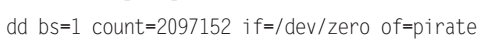
\includegraphics[scale=0.6]{images/lec05-pic01.png}
\end{figure}
Блок в 1024 байт:
\begin{figure}[h]
\centering
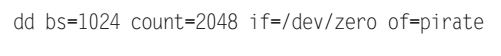
\includegraphics[scale=0.6]{images/lec05-pic02.png}
\end{figure}
\end{block}
\end{frame}

\begin{frame}{Ввод-вывод с пользовательским буфером}
\begin{figure}[h]
\centering
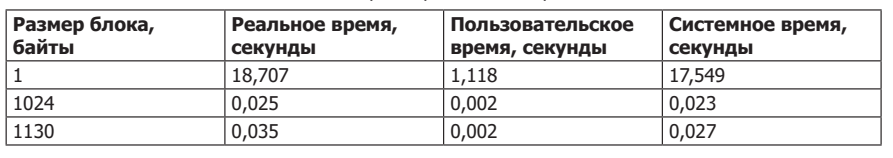
\includegraphics[scale=0.5]{images/lec05-pic03.png}
\end{figure}
\begin{itemize}
\item yа практике размер блока обычно составляет 512, 1024, 2048, 4096 или 8192 байт;
\item для значительного повышения производительности достаточно просто выполнять операции фрагментами, которые являются целочисленными кратными или делителями размера блока;
\item узнать размер блока на конкретном устройстве: системный вызов stat() или  команда stat(1).  
\end{itemize}
\end{frame}

\begin{frame}{Принцип работы пользовательского буфера}
Запись данных:
\begin{itemize}
\item по мере того как данные записываются, они сохраняются в буфере в пределах адресного пространства конкретной программы;
\item когда размер буфера достигает установленного предела, называемого размером буфера, содержимое этого буфера переносится на диск за одну операцию записи. 
\end{itemize}
Считывание данных:
\begin{itemize}
\item поступающие от приложения запросы на считывание имеют разные размеры и обслуживаются не из файловой системы напрямую, а удовлетворяются фрагментами,
получаемыми через буфер;
\item по мере того как приложение считывает все больше и больше информации, данные выдаются из буфера кусками;
\item как только буфер пустеет, начинается считывание следующего сравнительно крупного фрагмента, выровненного по границам блоков. 
\end{itemize}
\end{frame}

\subsection{Стандартный ввод-вывод}

\begin{frame}{Стандартный ввод-вывод}
\begin{itemize}
\item stdio - стандартная библиотека ввода-вывода Си; независимое от платформы решение для пользовательской буферизации. 
\item Си не содержит никакой встроенной поддержки ключевых слов для операций ввода-вывода. 
\item в процессе эволюции языка пользователи разработали стандартные наборы процедур, обеспечивающих основную функциональность - эти функции были объединены в стандартную библиотеку ANSI C (C89);
\end{itemize}
\begin{block}{Указатели файлов}
\begin{itemize}
\item Процедуры стандартного ввода-вывода используют свой уникальный идентификатор - указатель файла. 
\item В библиотеке C указатель файла ассоциируется с файловым дескриптором (отображается на него). 
\item Указатель файла представлен как указатель на определение типа FILE, определяемый в <stdio.h>.
\end{itemize}
\end{block}
\end{frame}

\subsection{Открытие файлов}
\begin{frame}{Открытие файлов}
\begin{figure}[h]
\centering
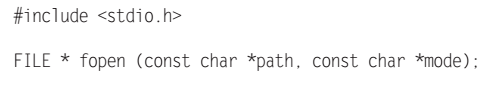
\includegraphics[scale=0.5]{images/lec05-pic04.png}
\end{figure}
Эта функция открывает файл \textit{path}, поведение которого определено в \textit{mode}, и ассоциирует с ним новый поток данных.

Возможные режимы отрытия файлы:
\begin{itemize}
\item \textbf{r} — файл открывается для чтения. Поток данных устанавливается в начале файла.
\item \textbf{r+} — файл открывается как для чтения, так и для записи. Поток данных устанавливается в начале файла.
\item \textbf{w} — файл открывается для записи. Если файл существует, то он усекается до
нулевой длины. Если файл не существует, он создается. Поток данных устанавливается в начале файла.
\end{itemize}
\end{frame}

\begin{frame}{Открытие файлов}
\begin{figure}[h]
\centering
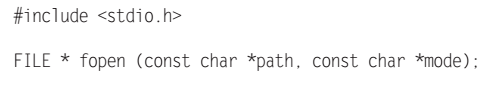
\includegraphics[scale=0.5]{images/lec05-pic04.png}
\end{figure}
\begin{itemize}
\item \textbf{w+} — файл открывается для чтения и для записи. Если файл существует, то он
усекается до нулевой длины. Если файл не существует, он создается. Поток
данных устанавливается в начале файла.
\item \textbf{a} — файл открывается для дополнения в режиме дозаписи. Если файл не существует, то он создается. Поток данных устанавливается в конце файла. Все вводимые данные дозаписываются в файл.
\item \textbf{a+} — файл открывается для дополнения и считывания в режиме дозаписи. Если файл не существует, то он создается. Поток данных устанавливается в конце файла. Все вводимые данные дозаписываются в файл.
\end{itemize}
\end{frame}

\begin{frame}{Открытие файлов}
\begin{itemize}
\item В случае успеха функция fopen() возвращает допустимый указатель FILE. 
\item При ошибке она возвращает NULL и устанавливает errno соответствующее значение
\end{itemize}
\begin{figure}[h]
\centering
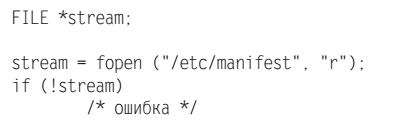
\includegraphics[scale=0.75]{images/lec05-pic05.png}
\end{figure}
\end{frame}

\begin{frame}{Открытие потока данных при помощи файлового дескриптора}
Функция fdopen() преобразует уже открытый файловый дескриптор (fd) в поток данных:
\begin{figure}[h]
\centering
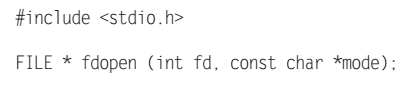
\includegraphics[scale=0.5]{images/lec05-pic06.png}
\end{figure}
\begin{itemize}
\item могут использоваться те же режимы, что и с функцией fopen(), при этом они должны быть совместимы с режимами, которые изначально применялись для открытия файлового дескриптора. 
\item режимы w и w+ можно указывать, но они не будут приводить к усечению файла. 
\item Поток данных устанавливается в файловую позицию, которая соответствует данному файловому дескриптору.
\item получить дексриптор - \textit{int fileno(FILE*stream)};
\end{itemize}
\end{frame}

\begin{frame}{Открытие потока данных при помощи файлового дескриптора}
Функция fdopen() преобразует уже открытый файловый дескриптор (fd) в поток данных:
\begin{figure}[h]
\centering
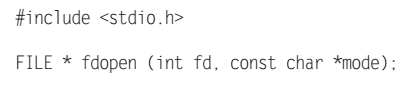
\includegraphics[scale=0.5]{images/lec05-pic06.png}
\end{figure}
\begin{itemize}
\item После преобразования файлового дескриптора в поток данных ввод-вывод больше не выполняется напрямую с этим файловым дескриптором. Тем не менее это не возбраняется. 
\item При закрытии потока данных закроется и файловый дескриптор.
\item В случае успеха fdopen() возвращает допустимый указатель файла, при ошибке она возвращает NULL и присваивает errno соответствующее значение.
\end{itemize}
\end{frame}

\begin{frame}{Открытие потока данных при помощи файлового дескриптора}
Например, следующий код открывает файл \textit{/home/kidd/map.txt} с помощью системного вызова \textit{open()}, а потом создает ассоциированный поток данных, опираясь на базовый файловый дескриптор:
\begin{figure}[h]
\centering
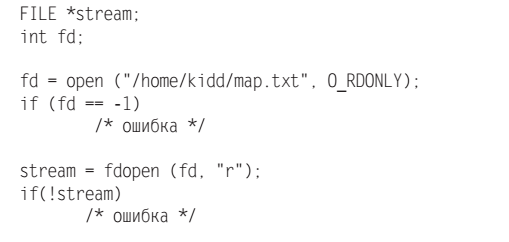
\includegraphics[scale=0.6]{images/lec05-pic07.png}
\end{figure}
\end{frame}

\subsection{Закрытие потоков данных}

\begin{frame}{Закрытие конкретного потока}
Функция \textit{fclose()} закрывает конкретный поток данных:
\begin{figure}[h]
\centering
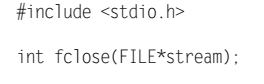
\includegraphics[scale=0.5]{images/lec05-pic08.png}
\end{figure}
\begin{itemize}
\item сначала сбрасываются на диск все буферизованные, но еще не записанные данные;
\item в случае успеха fclose() возвращает 0; 
\item При ошибке она возвращает EOF (конец файла) и устанавливает errno в соответствующее значение.
\end{itemize}
\end{frame}

\begin{frame}{Закрытие всех потоков данных}
Функция \textit{fcloseall()} закрывает все потоки данных, ассоциированные с конкретным процессом, в частности используемые для стандартного ввода, стандартного вывода и стандартных ошибок:
\begin{figure}[h]
\centering
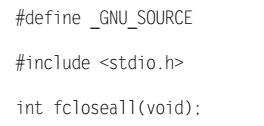
\includegraphics[scale=0.5]{images/lec05-pic09.png}
\end{figure}
\begin{itemize}
\item перед закрытием все потоки данных сбрасываются на диск;
\item функция является специфичной для Linux и всегда возвращает 0.
\end{itemize}
\end{frame}

\subsection{Считывание из потока данных}

\begin{frame}{Считывание одного символа в момент времени}
Функция \textit{fgetc()} используется для считывания отдельного символа из потока данных:
\begin{figure}[h]
\centering
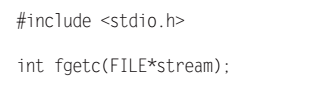
\includegraphics[scale=0.5]{images/lec05-pic10.png}
\end{figure}
\begin{itemize}
\item функция считывает следующий символ из stream и возвращает его как unsigned char, приведенный к int. 
\item такое приведение осуществляется, чтобы получить достаточно широкий диапазон для уведомлений EOF или описания ошибок: в таких случаях возвращается EOF
\item возвращаемое значение fgetc()должно быть сохранено в int. Сохранение в char — распространенный и опасный промах, ведь в таком случае вы не можете обнаруживать ошибки.
\end{itemize}
\end{frame}

\begin{frame}{Считывание одного символа в момент времени}
В следующем коде мы считываем отдельно взятый символ из stream, проверяем наличие ошибок и выводим результат как char:
\begin{figure}[h]
\centering
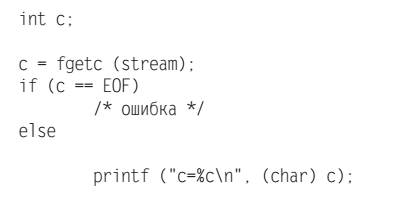
\includegraphics[scale=0.5]{images/lec05-pic11.png}
\end{figure}
\end{frame}

\begin{frame}{Возврат символа в поток данных}
 В рамках стандартного ввода­вывода предоставляется функция для перемещения символа обратно в поток данных. С ее помощью вы можете «заглянуть» в поток данных и возвратить символ обратно, если окажется, что он вам не подходит:
\begin{figure}[h]
\centering
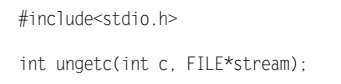
\includegraphics[scale=0.5]{images/lec05-pic12.png}
\end{figure}
\begin{itemize}
\item при каждом вызове мы отправляем обратно в поток данных stream символ c, приведенный к unsigned char. 
\item в случае успеха возвращается c, в случае ошибки — EOF.
\item если возвращаем в поток данных несколько символов - образуется стек
\item лишь один такой возврат должен гарантированно быть успешным (при отсутствии «вклинивающихся» запросов на считывание).
\end{itemize}
\end{frame}

\begin{frame}{Считывание целой строки}
Функция \textit{fgets()} считывает строку из указанного потока данных:
\begin{figure}[h]
\centering
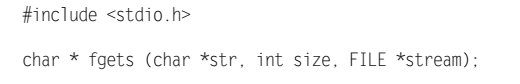
\includegraphics[scale=0.5]{images/lec05-pic13.png}
\end{figure}
\begin{itemize}
\item функция может считать из потока данных stream количество байтов, как максимум на один меньшее, чем количество size байт
\item результат считывания сохраняется в str.
\item символ нуля $\setminus 0$ сохраняется в буфере после последнего считанного байта. 
\item считывание прекращается, когда достигнут конец файла или первый символ новой строки. 
\item если начинается считывание новой строки, то в str сохраняется $\setminus n$.
\item В случае успеха возвращается str, в случае ошибки — NULL
\end{itemize}
\end{frame}

\begin{frame}{Считывание целой строки}
Пример:
\begin{figure}[h]
\centering
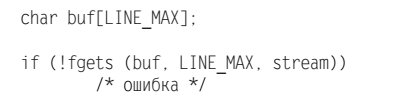
\includegraphics[scale=0.5]{images/lec05-pic14.png}
\end{figure}
\begin{itemize}
\item POSIX определяет LINE\_MAX в <limits.h>: это максимальный размер, который может иметь строка ввода, чтобы интерфейсы POSIX для манипуляций со строками могли ею оперировать. 
\item В библиотеке C такое ограничение отсутствует — строки могут быть любого размера.
\end{itemize}
\end{frame}

\begin{frame}{Считывание двоичных данных}
Для того, чтобы считывать и записывать сложные двоичные данные, в частности структуры Cи, предоставляется функция \textit{fread()}:
\begin{figure}[h]
\centering
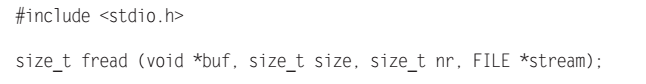
\includegraphics[scale=0.5]{images/lec05-pic15.png}
\end{figure}
\begin{itemize}
\item При вызове fread() мы можем прочитать вплоть до nr фрагментов данных, каждый размером size байт. 
\item Считывание происходит из потока данных stream в буфер, указанный buf. 
\item Значение файлового указателя увеличивается на число, равное количеству прочитанных байтов.
\item Возвращается количество считанных элементов (но не количество считанных
байтов!). 
При ошибке или достижении конца файла функция возвращает значение,
меньшее чем nr. К сожалению, мы не можем узнать, какое именно из двух условий
наступило, — для этого потребуется специально применить функции ferror() и feof()
\end{itemize}
\end{frame}

\begin{frame}{Считывание двоичных данных}
Для того, чтобы считывать и записывать сложные двоичные данные, в частности структуры Cи, предоставляется функция \textit{fread()}:
\begin{figure}[h]
\centering
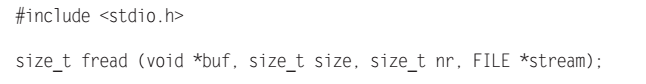
\includegraphics[scale=0.5]{images/lec05-pic15.png}
\end{figure}
\begin{itemize}
\item gри ошибке или достижении конца файла функция возвращает значение, меньшее чем nr. 
\item К сожалению, мы не можем узнать, какое именно из двух условий наступило, — для этого потребуется специально применить функции ferror() и feof().
\end{itemize}
\end{frame}

\begin{frame}{Считывание двоичных данных}
Простейший образец fread() применяется для считывания одного элемента линейных байтов из указанного потока данных:
\begin{figure}[h]
\centering
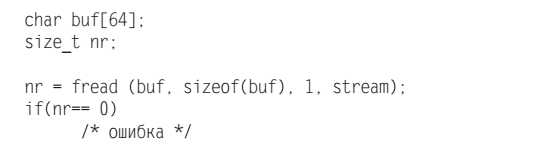
\includegraphics[scale=0.75]{images/lec05-pic16.png}
\end{figure}
\end{frame}

\subsection{Запись в поток данных}

\begin{frame}{Запись отдельного символа}
Функция, парная fgetc(), называется fputc():
\begin{figure}[h]
\centering
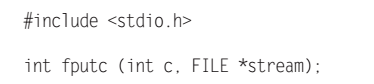
\includegraphics[scale=0.75]{images/lec05-pic17.png}
\end{figure}
\begin{itemize}
\item Функция fputc() записывает байт, указанный в c (приведенный к unsigned char),
в поток данных, указанный в stream. 
\item При успешном завершении операции функция возвращает c. В противном случае она возвращает EOF и присваивает errno соответствующее значение.
\end{itemize}
\begin{figure}[h]
\centering
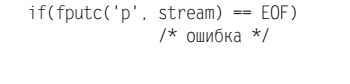
\includegraphics[scale=0.75]{images/lec05-pic18.png}
\end{figure}
\end{frame}

\begin{frame}{Запись строки символов}
Функция fputs() используется для записи целой строки в заданный поток данных:
\begin{figure}[h]
\centering
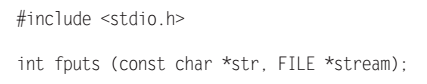
\includegraphics[scale=0.75]{images/lec05-pic19.png}
\end{figure}
\begin{itemize}
\item при вызове fputs() все содержимое строки, оканчивающейся нулем, записывается в поток данных, указанный в stream.
\item сама эта строка указывается в str. 
\item в случае успеха fputs() возвращает неотрицательное число. При ошибке она возвращает EOF.
\end{itemize}
\end{frame}

\begin{frame}{Запись строки символов}
В следующем примере файл открывается для внесения данных в режиме дозаписи. Указанная строка записывается в ассоциированный поток данных, после чего
этот поток данных закрывается:
\begin{figure}[h]
\centering
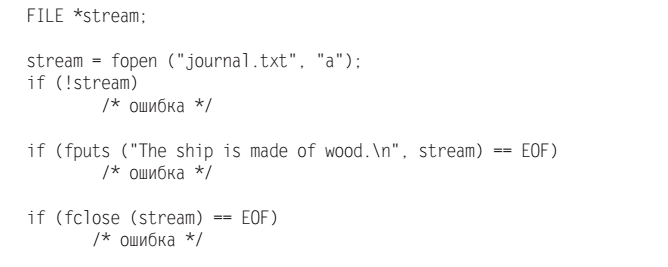
\includegraphics[scale=0.75]{images/lec05-pic20.png}
\end{figure}
\end{frame}

\begin{frame}{Запись двоичных данных}
Для непосредственного сохранения двоичных данных, например переменных языка C, в рамках стандартного ввода­вывода предоставляется функция fwrite():
\begin{figure}[h]
\centering
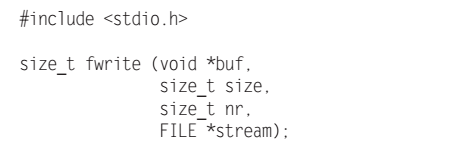
\includegraphics[scale=0.6]{images/lec05-pic21.png}
\end{figure}
\begin{itemize}
\item при вызове fwrite() в поток данных stream записывается вплоть до nr элементов,
каждый до size в длину. 
\item Берутся данные из буфера, указанного в buf. 
\item Значение файлового указателя увеличивается на число записанных \textbf{байтов}.
\item Возвращается количество успешно записанных \textbf{элементов}. 
\item  Возвращаемое значение меньше nr означает ошибку.
\end{itemize}
\end{frame}

\subsection{Позиционирование в потоке данных}

\begin{frame}{Позиционирование в потоке данных}
Функция fseek(), наиболее распространенный интерфейс позиционирования из инструментов стандартного ввода­вывода,
управляет файловой позицией в потоке данных stream в зависимости от значений offset и whence:
\begin{figure}[h]
\centering
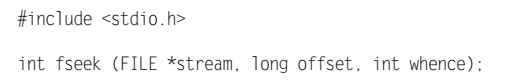
\includegraphics[scale=0.6]{images/lec05-pic22.png}
\end{figure}
\begin{itemize}
\item Если аргумент whence имеет значение SEEK\_SET, то файловая позиция устанавливается в offset. 
\item Если whence равен SEEK\_CUR, файловая позиция получает значение, равное «текущая позиция плюс offset». 
\item Если whence имеет значение SEEK\_END, то файловая позиция устанавливается в значение, равное «конец файла плюс
offset».
\end{itemize}
\end{frame}

\begin{frame}{Позиционирование в потоке данных}
Функция fseek(), наиболее распространенный интерфейс позиционирования из инструментов стандартного ввода­вывода,
управляет файловой позицией в потоке данных stream в зависимости от значений offset и whence:
\begin{figure}[h]
\centering
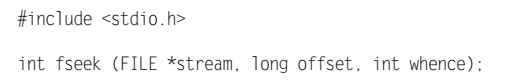
\includegraphics[scale=0.6]{images/lec05-pic22.png}
\end{figure}
\begin{itemize}
\item При успешном завершении функция fseek() возвращает 0, стирает индикатор EOF и отменяет любые эффекты функции ungetc() (при их наличии). 
\item При ошибке она возвращает –1 и устанавливает errno в соответствующее значение. 
\item Самые распространенные ошибки — это недействительный поток данных (EBADF) и недействительный аргумент whence (EINVAL).
\end{itemize}
\end{frame}

\begin{frame}{Получение актуальной позиции в потоке данных}
Функция ftell() возвращает текущую позицию из потока данных stream:
\begin{figure}[h]
\centering
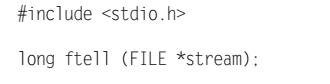
\includegraphics[scale=0.6]{images/lec05-pic23.png}
\end{figure}
\begin{itemize}
\item При ошибке она возвращает –1 и устанавливает errno в соответствующее значение.
\end{itemize}
\end{frame}

\subsection{Сброс потока данных}

\begin{frame}{Позиционирование в потоке данных}
В стандартной библиотеке ввода­вывода есть интерфейс, позволяющий выписать
содержимое пользовательского буфера в ядро. 

Он гарантирует, что все данные, записанные в поток данных, будут сброшены к ядру с помощью write().
\begin{figure}[h]
\centering
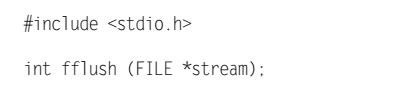
\includegraphics[scale=0.6]{images/lec05-pic24.png}
\end{figure}
\begin{itemize}
\item При вызове этой функции все незаписанные данные из потока данных, указанного в stream, сбрасываются в буфер ядра. 
\item Если значение stream равно NULL, то все открытые потоки данных этого процесса записываются в буфер ядра. 
\item В случае успеха fflush() возвращает 0. 
\item В случае ошибки эта функция возвращает EOF и присваивает errno соответствующее значение.
\end{itemize}
\end{frame}

\subsection{Обработка ошибок}

\begin{frame}{Ошибки и конец файла}
Проверика статуса конкретного потока данных и определение, установлен ли на потоке данных
stream индикатор ошибки:
\begin{figure}[h]
\centering
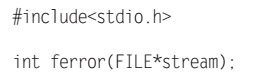
\includegraphics[scale=0.6]{images/lec05-pic25.png}
\end{figure}
Функция feof() проверяет, установлен ли на потоке данных stream индикатор
EOF:
\begin{figure}[h]
\centering
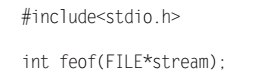
\includegraphics[scale=0.6]{images/lec05-pic26.png}
\end{figure}
Функция clearerr() удаляет с потока данных stream индикаторы ошибки и EOF:
\begin{figure}[h]
\centering
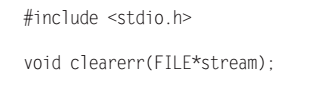
\includegraphics[scale=0.6]{images/lec05-pic27.png}
\end{figure}
\end{frame}

\begin{frame}{Выводы}
Стандартный ввод-вывод и пользовательская буферизация оправданны, если выполняются все следующие условия:
\begin{itemize}
\item предположительно вы будете делать много системных вызовов и хотите минимизировать сопутствующие издержки, объединив несколько таких вызовов в один;
\item очень важна высокая производительность, и вы хотите гарантировать, что весь
ввод­вывод будет осуществляться поблочными фрагментами, четко ограниченными размерами блоков;
\item интересующие вас шаблоны доступа основаны на символах или строках, и вам
нужны интерфейсы, обеспечивающие такой доступ без выполнения излишних системных вызовов;
\item вы предпочитаете использовать сравнительно высокоуровневый интерфейс, а не
низкоуровневые системные вызовы Linux.
\end{itemize}
Однако максимальная гибкость обеспечивается, когда вы работаете непосредственно с системными вызовами Linux.
\end{frame}

\end{document}
